\section{背景}
本プロジェクトでは、「視覚や聴覚に頼れない状況で役立つ装置の開発」をコンセプトとし、障害者が抱える問題を当事者目線で検討し、実用的な装置の開発に取り組んできた。頼れない感覚を別の手段で補うことで、不便を解消し、安全で快適な生活を支援することを目指している。
聴覚障害や視覚障害、色覚の障害者を対象とした4つのグループに分かれ、それぞれ、特定の言葉や音に反応するデバイス、画像の色をユニバーサルデザインに変換するアプリ、自力で避難することが難しい人のための補助デバイス、障がい者が自然を楽しむためのデバイスの開発を行っている。

\section{課題の設定と到達目標}
\subsection{Group A: 色覚班}
色覚異常を持つ人々は、特定の色の組み合わせを見分けることができず、必要な情報を得られないことがある。
そこで、色覚異常を持つ人々が判別しにくい色を判別しやすくすることを目的とし、容易にユニバーサルカラーに変換することのできるアプリケーションの開発を行う。

\subsection{Group B: 聴覚支援班}
高齢者や中途失聴者などの聴覚障害者は、孤立しやすく、難聴であることを周囲に知られたくないという懸念を抱えている。
そこで、周囲に気づかれることなく、自身への呼びかけに気づけるよう補助し、孤立や不安を軽減するデバイスの開発を行う。

\subsection{Group C: 災害支援班}
視覚障害者・聴覚障害者などの、災害時に自力での避難が困難な避難行動要支援者が多数おり、避難時に置き去りなどの問題が発生している。
そこで、災害時において、避難行動要支援者が周囲の人々に助けを求めることを補助し、避難における自助・共助を行うことのできるデバイスの開発を目指す。

\subsection{Group D: 自然エンタメ班}
風の音や木々の揺れなど、日常的に自然の楽しさを体感している。
しかし、視覚や聴覚に障害のある方はそれが難しいと考えた。
自然を誰でも楽しめるようにしたい。
そこで、視覚や聴覚情報の相互変換を可能にするデバイスを開発し、障害の有無に関わらず誰でも自然を楽しめるようにし、自然の新たな楽しみ、価値をデザインする。

\section{課題解決のプロセスとその結果}
\subsection{Group A: 色覚班}

\subsection{Group B: 聴覚支援班}
\subsubsection{対象者と問題の提示}
対象者は聴覚障害者で、特に呼びかけに気づけないことで社会参加が難しくなるという問題に直面している。この問題は、精神的な負担や孤立感を引き起こす要因となっている。
\subsubsection{使用技術の選定}
音声認識技術を選定し、特定の言葉を認識して振動通知を行うシステムを構築することとした。これにより、聴覚に頼らず通知を受け取ることが可能となる。
\subsubsection{システム構築}
既存の音声認識ツールを活用して、名前や呼びかけの言葉を認識し、それに反応して振動するシステムを構築した。これにより、実装の効率化を図ることができた。
\subsubsection{デバイスデザインの考案}
デバイスは目立たず、使いやすいデザインにすることが重要とされ、装着者が違和感なく使用できるように配慮した。デザインは日常的に着用できる軽量でコンパクトな形状を目指した。
\subsubsection{成果物}
成果物として、音声認識に反応して振動通知を行うデバイスを完成させた。このデバイスは、聴覚障害者が社会的に孤立することを防ぎ、日常生活でのコミュニケーションをサポートする。
\begin{figure}[h]
  \centering
  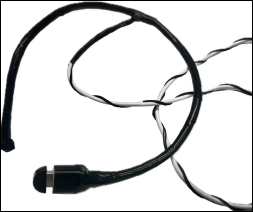
\includegraphics[width=0.45\textwidth]{pages/report/images/Choukakudevice.jpg}
  \caption{聴覚支援班:成果物}
  \label{fig:Choukakudevice}
\end{figure}
\subsection{Group C: 災害支援班}

\subsection{Group D: 自然エンタメ班}
目的を達成するために、RaspberryPiを用いたカメラ型デバイス「オトフォトン」を作成し、写真と音の相互変換を行う。
具体的には、撮った写真に応じた音楽を選曲し再生する機能と、録音した環境音を元にビジュアルアートを生成する機能を実装した。
また、デジタルデバイドを考慮し、誰でも扱いやすいデジタルカメラに寄せたデザインにした。

\begin{figure}[h]
  \centering
  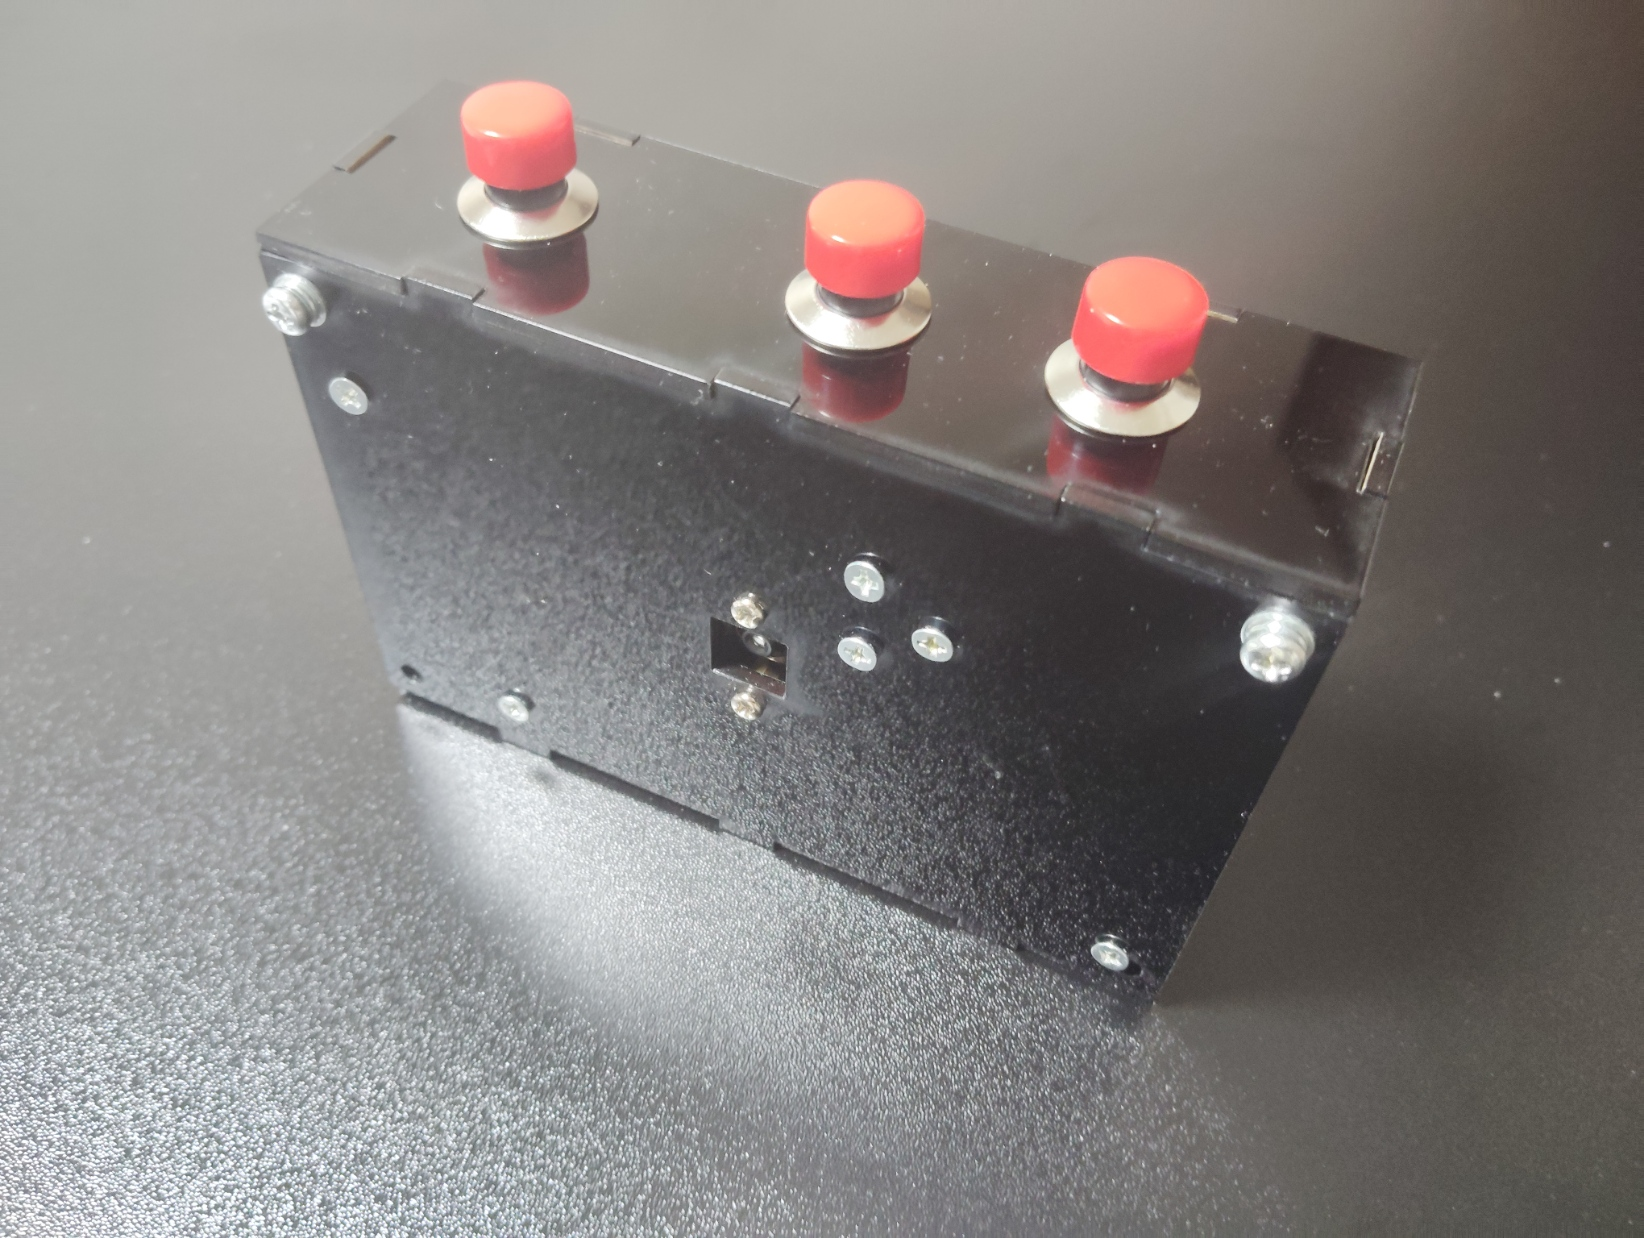
\includegraphics[width=0.45\textwidth]{pages/report/images/otophoton.jpg}
  \caption{オトフォトン}
  \label{fig:otophoton}
\end{figure}

\section{結論と展望}
\subsection{Group A: 色覚班}

\subsection{Group B: 聴覚支援班}
本研究のデバイスは、聴覚障害者が他者の呼びかけに気づくための有効なツールとなり得ると考える。今後は、認識精度の向上やデバイスの更なる小型化、使いやすさの改善を進め、より多くの聴覚障害者に役立つことを目指す。
\subsection{Group C: 災害支援班}

\subsection{Group D: 自然エンタメ班}
音楽やビジュアルアートを好みに応じてカスタマイズできる機能等、細かな機能の追加をしたい。
また、このデバイスによって、自然の新たな楽しみ方を実現し、新しい価値をデザインしていきたい。
